\section{What is this?}

This is the script for the 'Stars and Elementary Astrophysics' (SEA) lectures, which are part of AS1001. The script covers the \textit{skeleton of facts} for this course, including important equations and numbers. \textit{It is not a replacement for taking notes at the lectures.} The lectures will cover everything in this script, but with more illustrations, explanations, figures, animations, and examples. The slides from the lectures will \textit{not} be on Moodle. Important terms and concepts are marked with italics. Important equations are in bold. The textbook for this course is Kutner's 'Astronomy - A Physical Perspective'. 

Synopsis: SEA answers the basic question 'what is a star?'. This includes measuring distances to stars, and finding out how large, hot, massive stars are. SEA also covers the essential toolkit for astronomers - telescopes and instruments - as well as the basics of electromagnetic radiation. \textit{SEA is the fundament for all other astronomy modules.}

\section{Introduction}

Astronomy is: the study of the stars. But astronomy also covers planets, gas clouds, galaxies, black holes, pulsars, the Universe itself - so, \textit{everything in the material world except things on Earth}.

Astronomy needs physics, chemistry, mathematics (and perhaps biology?).

\textit{What is a star?} To the eye, stars are points of light at the night sky. They are grouped in \textit{constellations} - these are arbitrary groupings of stars, which means: chance projections, no physical groups. Today only meaningful to 'find your way' on the sky. Examples for well-known constellations are Orion, Ursa Major, Taurus, Cassiopeia. 

The constellations that are visible change over the year (due to the rotation of the Earth around the Sun) and over the night (due to the rotation of the Earth). 

Looking at the night sky shows: stars have different brightnesses, colours, positions. \textit{But what is a star really?}

\section{Distances to stars}

Fundamental problem: A point of light at the sky could be a nearby candle or a very distant supernova. To find out what stars really are, we need a method to determine the distance that is independent of the brightness. The most important method in this context is the \textit{parallax}.

\subsection{Parallax}

The parallax method is based on \textit{triangulation}. The basic principle is explained in Fig. 1. If we can measure the angle p and the baseline s in the triangle, we can infer the distance: $\tan{(p)} = s/d$, i.e. $d = s/\tan{(p)}$. For small $p$, we can use the small angle approximation, $\tan{(tp)} \sim p$. That means:

\begin{equation}
d = s/p
\end{equation}

In astronomy, $p$ (the parallax) is measured in \textit{arcseconds} (arcsec). 1" = 1 arcsec = 1/3600th of one degree. This is a very small angle.

\begin{figure}[h]
\begin{center}
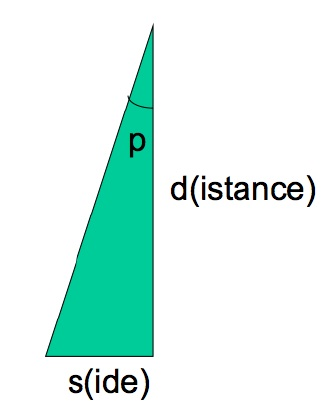
\includegraphics[width=5cm]{sea_fig1.jpg}
\end{center}
\end{figure}

\subsection{The parsec}

A \textit{parsec} is defined as the distance of an object that has a parallax of 1 arcsec. Fig. 2 illustrates the idea. The semi-major axis of the Earth's orbit is $1.5 \cdot 10^{11}$\,m (defined as 1\,Astronomical Unit). If the parallax is measured in arcsec, the distance $d$ to the star from the Sun in units of parsec is simply:

\begin{equation}
d = 1/p
\end{equation}

What is 1\,pc in metric units? Start with Equ 1, $d = s/p$. Use $s = 1\,\mathrm{AU} = 1.5 \cdot 10^{11}$\,m. 1\,pc distance means $p = 1" = (1/3600)$ degrees. Convert this to radians and put in Equ 1: $d = 1.5 \cdot 10^{11} / 0.0000048 = 3.1 \cdot 10^{16}$\,m. 

The closest stars to the Sun are at 1.3\,pc (and a parallax of 0.75" the $\alpha$\,Centauri system (a triple star). There are several hundred stars within 10\,pc, among them Sirius, Vega, Procyon, Altair, some of the brightest stars on the sky.

\subsection{Measuring the parallax}

How accurately can we measure positions of stars? Parallaxes are very small angles! First successful measurements in 1838-1839. Today, 0.05" can be done with ground-based telescopes. The satellite Hipparcos (1989-1993) measured parallaxes for 100.000 stars with 0.001" accuracy. The satellite Gaia (2013+) will get parallaxes for one billion stars with 0.0001" accuracy - this is still only 1\% of the stars in the Milky Way.

This means: The parallax only covers our cosmic neighbourhood. We need other methods for objects at larger distances. There are many more methods to determine distances of stars, some will be discussed in other parts of SEA1001. But all are based on the parallax.

\section{Brightness of stars}

\subsection{Flux and luminosity}

The \textit{luminosity} $L$ is the total energy emitted by a star per seconds, i.e. it is measured in Joule/sec or Watts. On Earth we only receive a part of this energy. The \textit{flux} $f$ is the energy per second that an observer on Earth measures. \textit{Luminosity is what the source emits, flux is what the observer receives.}

\subsection{Inverse square law for the propagation of light}

Flux and luminosity are related through the basic law that describes the propagation of light. The light from a star spreads out \textit{isotropically} (i.e. the same amount in all directions) over the surface of a sphere(see Fig. 3). The flux is therefore:

\begin{equation}
f = L / (4 \pi d^2)
\end{equation}

Example: Assume a detector measure f=1 for a star. Now we move the detector further away. At twice the distance, the light from the star has spread out to cover four times the surface, i.e. a light detector with a fixed area collects 1/4 of the light. The flux drops with the inverse square of the distance.

Equ 3 contains three quantities, flux, luminosity and distance. The flux can be measured on Earth. The inverse square law can be used to determine luminosities, if the distance is known (from the parallax). can be used to determine distances, if the luminosity of a star is known. It can also be used to determine distances, if the luminosity of a star is known. This second aspect leads to the concept of standard candles.

\subsection{Standard candles and cepheids}

A \textit{standard candle} is an astronomical object with a known brightness, i.e. we know in some way how much light it emits. From this and the measured flux the distance can be derived using the inverse square law. Standard candles usually have properties that do not vary with distance.

\textit{Cepheids} are one example for standard candles. These are supergiant stars which vary in brightness due to pulsation. Their pulsation period and their luminosity are related - the longer the period the larger the luminosity (see Fig. 4). From the period and the flux the distance can be derived.

\subsection{Units for the brightness of stars}

The unit of the flux is Watts per square meter. This is very small for astronomical objects. Often used instead: unit 'Jansky' which is defined as $1\,Jy = 10^{-26}$\,W\,m$^{-2}$\,Hz$^{-1}$

Flux is measured on a linear scale, i.e. a source of 10\,Jy is ten times brighter than a source of 1\,Jy. This is inconvenient in astronomy, more useful would be a logarithmic scale $\log{(f)}$. This leads to the concept of magnitudes.

\subsection{Magnitudes}

The unit magnitudes is derived from a system first used by the Greek astronomer Hipparcox (2nd century BC). In his catalogue of stars, 1st magnitude are the brightest stars, 6th magnitude are the stars just visible for the human eye. This system has now been adopted and extended for modern astronomy. The relation between fluxes and magnitudes is:

\begin{equation}
m_1 - m_2 = -2.5 \log{(f_1 / f_2)}
\end{equation}

Or conversely:

\begin{equation}
f_1 / f_2 = 10^{(m_1 - m_2) / -2.5}
\end{equation}

This is a logarithmic system, but with a scaling factor of 2.5. This factor means that 5\,mag difference correspond to a factor of 100 in flux. The zeropoint for the magnitude scale is Vega at $m = 0.0$.

\subsection{Magnitudes and distances}

Usually magnitudes are \textit{apparent magnitudes} (donated with small letter $m$). They relate to the flux measured on Earth and depend (as the flux does) on the distance. 

But we can also define a magnitude that relates to the luminosity and do not depend on distance. This is the \textit{absolute magnitude} (donated with capital letter $M$). The absolute magnitude is the magnitude a star would have at a distance of 10\,pc. Substituting Equ 3 into Equ 4 gives $m - M = -2.5 \log{ (10 / d)^2 } =   -2.5 \cdot -2 \log{(d/10)}$, i.e.:

\begin{equation}
m - M = -5 \log{(d/10\,\mathrm{pc})}
\end{equation}

The quantity $m-M$ is called the \textit{distance modulus} and is another unit for distances of stars. If the distance of a star is known, the apparent magnitude $m$ can be measured and the absolute magnitude $M$ can be derived. 

\section{Binary stars}

\textit{Binary stars} are systems which are very useful when determining stellar masses and sizes. Binaries are two stars in mutual gravitational interaction orbiting their common center of mass (see Fig. 5). Higher order binaries like triples and quadruples exist as well. Most stars are born as multiples.

We distinguish:
\begin{itemize}
\item{\textit{Visual binaries}: Two stars are seen separately}
\item{\textit{Spectroscopic binaries}: Stars are not seen separately, but the spectrum shows two set of lines moving in opposite directions due to the Doppler shift.}
\item{\textit{Eclipsing binaries}: Stars are not seen separately, but one star eclipses the other in regular intervals.}
\end{itemize}

Binaries are useful for two reasons: a) Orbits determined by gravity, i.e. they can be used to determine masses. b) Eclipses determined by sizes, i.e. can be used to determine radii. Eclipsing binaries are therefore important to determine the fundamental properties of stars (i.e. what a star really is).

\subsection{Doppler effect}

The wavelength that an observer measures depends on the relative motion between the observer and the light source. If the source is moving towards the observer, the light is blueshifted ($\lambda < \lambda_0$). If the source is moving away from the observer, the light is redshifted ($\lambda >\lambda_0$). This is called the \textit{Doppler effect} (analogous to the Doppler effect with sound waves).

The shift in wavelength due to the Doppler effect in the light of a star is this:

\begin{equation}
\Delta\lambda / \lambda = v/c
\end{equation}

Here $c$ is the speed of light, $Delta\lambda$ is the wavelength difference $(\lambda - \lambda_0)$, and $v$ is the \textit{radial velocity} of the star, i.e. the relative speed of the star along the line of sight of the observer. Equ 8 is only valid for $v<<c$.

The Doppler effect shifts lines in the spectra of stars (see Sect. XXX). From these shifts and with Equ 8 the radial velocities of stars can be measured. The Doppler effect has many applications in astronomy; one example is the study of binary stars.

\subsection{Orbits of binaries}

Fig. XXX shows the orbit for a binary. We consider here circular orbits for simplicity. The orbital period is $P = 2 \pi r / v$. In the system $P_1 = P_2$. From these two equations follows:

\begin{equation}
r_1 / v_1 = r_2 / v_2
\end{equation}

With the definition of the center of mass $m_1 r_1 = m_2 r_2$ we obtain:

\begin{equation}
v_1 / v_2 = r_1 / r_2 = m_2 / m_1
\end{equation}

This means, the more massive star is orbiting at a shorter distance from the center of mass and with a smaller velocity.

\subsection{Kepler's 3rd law for binaries}

Newton's law of gravity is: $F = G m_1 m_2 / (r_1 + r_2)^2$

The gravitational force equals the force to keep the star in orbit: 

\begin{equation}
m_1 v_1^2 / r_1 = G m_1 m_2 / (r_1 + r_2)^2
\end{equation}

With $v_1 = 2 \pi r_1 P$ follows $4 \pi^2 r_1 / P^2 = G m_2 (r_1 + r_2)^2$. With $R = r_1 + r_2$ (see textbook) this gives:

\begin{equation}
4 \pi^2 R^3 / G = (m_1 + m_2) P^2
\end{equation}

In solar system units (distance between the stars in AU, period in years, masses in solar masses), this equation simplifies to:

\begin{equation}
a^3 = (m_1 + m_2) P^2
\end{equation}

This is \textit{Kepler's 3rd law}. 

In a spectroscopic system, the radial velocities $v_1$ and $v_2$ can be measured, together with the period. This immediately gives $r_1$ and $r_2$ and thus $R$, as well as the ratio $m_1$ and $m_2$. With Kepler's 3rd law, we can calculate the sum of the masses. Together this gives individual masss for the components. Factors that are neglected here: elliptic orbits, inclination of orbits against the line of sight (for spectroscopic binaries) or the sky (for visual binaries). 

\subsection{Eclipsing binaries}

Fig. XXX shows the lightcurve of an eclipsing binary system. From the lightcurve, $t_1$, $t_2$, $t_3$, $t_4$ can be measured. The geometry of the system then gives expressions for the radii $R_1$ and $R_2$ of the stars:

\begin{equation}
t_4 - t_1 / P = (R_1 + R_2) / (2 \pi R)
\end{equation}

\begin{equation}
t_3 - t_2 / P = (R_1 - R_2) / (2 \pi R)
\end{equation}

With these two equations the radii can be derived in units of the orbital separation $R$. The radial velocities $v$ and the period $P$ yield $R$, and thus the radii of the stars. This only works in an eclipsing binary which is also a spectroscopic binary. This rare type of system is therefore extremely important in astronomy.

\section{Synopsis}

\subsection{Properties of stars}

Observable properties: position, flux, magnitude, colour, spectrum, spectral type, lightcurve

Physical properties: luminosity, velocity, absolute magnitude, size, mass, temperature

Astronomy means finding clever methods to get physical properties from observable properties.

